\documentclass{beamer}
\mode<presentation> {
\usetheme{Madrid}
}

\usepackage{amsmath,amsthm,amssymb,amsfonts,cancel}
\usepackage{graphicx} % Allows including images
\usepackage{color}

\usepackage{booktabs} % Allows the use of \toprule, \midrule and \bottomrule in tables
\usepackage{caption}
\usepackage{algorithm} 
\usepackage{algpseudocode}
%\usepackage[style=verbose, backend=bibtex,maxcitenames=4]{biblatex}
%\addbibresource{references.bib}
%{\footnotesize
%\bibliography{references}}

%%change footnotecite
%\renewcommand*{\thefootnote}{[\arabic{footnote}]}
%\makeatletter
%% Remove superscript for footnotemark
%\def\@makefnmark{\hbox{{\normalfont\@thefnmark}}}
%% Allow space to precede the footnote
%\usepackage{etoolbox}
%\patchcmd{\blx@mkbibfootnote}{\unspace}{}{}
%\makeatother

%\setbeamertemplate{bibliography item}{}
\setbeamertemplate{theorems}[numbered]
\newtheorem{thm}{Theorem}
\newtheorem{lem}[thm]{Lemma}
\newtheorem{cor}{Corollary}
\newtheorem*{defi*}{Definition}

\title[]{Local Distance Correlation For Testing Independence} 

\author{Cencheng Shen} % Your name
\institute[Temple University] % Your institution as it will appear on the bottom of every slide, may be shorthand to save space
{
\textit{Joint Work with Joshua T. Vogelstein \& Carey E. Priebe} \\
%\medskip
%Department of Statistics \\
%Temple University \\  % Your institution for the title page
}
\date{November 19, 2015} % Date, can be changed to a custom date

\AtBeginSection{\frame{\sectionpage}}

\begin{document}

\begin{frame}
\titlepage % Print the title page as the first slide
\end{frame}
%1. Intro; 2. it is linear regression and classification; 3. its origin, and why we start investigation; 4. explain title

\begin{frame}
\frametitle{Overview} % Table of contents slide, comment this block out to remove it
\tableofcontents % Throughout your presentation, if you choose to use \section{} and \subsection{} commands, these will automatically be printed on this slide as an overview of your presentation
\end{frame}

\section{Motivations}
\begin{frame}{Motivations}
\begin{itemize}[<+->]
\item Given multiple data sets, we would like to test whether they are independent or not.
\item Modern data sets may be high-dimensional, nonlinear, noisy, of small sample size; and different data sets may come from disparate spaces.
\item One example we have is Brain Connectome vs Personality: the Brain Connectome is measured on $197$ brain regions for $194$ time steps, and the personality data is a five-factor model. The sample size is $42$.
\item Initially we tried various regression methods on the data in order to predict personality from Connectome, but it does not work...  
\end{itemize}
\end{frame}
%tba: emphasize second point

\begin{frame}
\begin{itemize}[<+->]
\item So we decide to test whether the two data sets are independent or not: if they are independent, then there is no point to do prediction.
\item The basic question is: \textbf{How to test independence on real data???}
\item The Pearson correlation coefficient and RV coefficient are mostly useful for finding linear relationship and may be zero for dependent data sets, while mutual information requires estimating the probability distribution.
\end{itemize}
\end{frame}

\begin{frame}
\begin{itemize}[<+->]
\item We turn to a great method in the Statistical community: \textbf{distance correlation}.
\item It is easy to compute for given data in Euclidean space, and is a consistent test statistic with good simulation results \cite{SzekelyRizzoBakirov2007}.
\item But it does not work well against high-dimensional and non-linear dependency. 
\item And its theoretical consistency is not equivalent to good finite-sample testing power: the sample size may be limited due to expensive data collection, while the required sample size to achieve good power for a particular dependency type can be very large.
\item Most importantly, it fails to detect any relationship in our Connectome vs personality data.
\end{itemize}
\end{frame}

\begin{frame}
\begin{itemize}[<+->]
\item There exists other methods in the same distance-based framework: 
\item Modified distance correlation \cite{SzekelyRizzo2013a} is robust against high-dimensionality, but still not nonlinear data. 
\item The HHG statistic \cite{HellerGorfine2013} works well for nonlinear data, but falls a bit short in linear and high-dimensional data.
\item The kernel-based independence test developed in \cite{GrettonGyorfi2010} is a similar tool in the machine learning community, whose connection to distance correlation is established in \cite{SejdinovicEtAl2013}.
\end{itemize}
\end{frame}

\section{Global Distance Correlation}
\begin{frame}{Set-Up}
\begin{itemize}[<+->]
\item Given two data sets $\mathcal{X}=[X_{1},\cdots, X_{n}] \in \mathcal{R}^{m_{X} \times n}$ and $\mathcal{Y}=[Y_{1},\cdots, Y_{n}] \in \mathcal{R}^{m_{Y} \times n}$, \item Assume that $X_{i}, i=1,\ldots,n$ are identically independently distributed (i.i.d.) as $X$, similarly $Y_{i} \stackrel{i.i.d.}{\sim} Y$. 
\item For testing independence between $X$ and $Y$, the null and the alternative hypothesis are
\begin{align*}
& H_{0}: X \mbox{ is independent of } Y, i.e., f_{XY}=f_{X}f_{Y},\\
& H_{A}: f_{XY} \neq f_{X}f_{Y},
\end{align*}
where $f_{XY}$ denotes the joint distribution of $(X,Y) \in \mathcal{R}^{m_{X}+m_{Y}}$, and $f_{X}$ and $f_{Y}$ are the marginal distributions. 
\end{itemize}
\end{frame}

\begin{frame}{Distance Covariance}
\begin{itemize}[<+->]
\item Since the random variables are not directly observed, we test by the sample data $\mathcal{X}$ and $\mathcal{Y}$.
\item We first calculate two Euclidean distance matrices $A, B \in \mathcal{R}^{n \times n}$ for $\mathcal{X}$ and $\mathcal{Y}$ respectively, i.e., $A_{ij}=\|X_{i}-X_{j}\|_{2}$. 
\item The sample distance covariance is defined as
\begin{equation}
\label{dCovEqu}
dCov_{n}(\mathcal{X},\mathcal{Y})=\frac{1}{n^2}\sum_{i,j=1}^{n}A^{H}_{ij}B^{H}_{ij},
\end{equation}
where $A^{H}=HAH$, $B^{H}=HBH$ with $H=I_{n}-\frac{J_{n}}{n}$. 
\item Then the sample distance variance is defined as
\begin{align*}
dVar_{n}(\mathcal{X}) &=\frac{1}{n^2}\sum_{i,j=1}^{n}A^{H}_{ij}A^{H}_{ij}\\
dVar_{n}(\mathcal{Y}) &=\frac{1}{n^2}\sum_{i,j=1}^{n}B^{H}_{ij}B^{H}_{ij}.
\end{align*}
\end{itemize}
\end{frame}

\begin{frame}{Distance Correlation}
The squared sample distance correlation is obtained by normalizing the distance covariance
\begin{equation}
\label{dCorrEqu}
dCorr_{n}(\mathcal{X},\mathcal{Y})=\frac{dCov_{n}(\mathcal{X},\mathcal{Y})}{\sqrt{dVar_{n}(\mathcal{X}) \cdot dVar_{n}(\mathcal{Y})}},
\end{equation}
where all of $dCov_{n}, dVar_{n}, dCorr_{n}$ are always non-negative. 
\end{frame}

\begin{frame}{Consistency of Distance Correlation}
\begin{thm} 
As $n \rightarrow \infty$, the sample distance correlation converges to $0$ if and only if the null hypothesis is true, i.e., $X$ is independent of $Y$.
\end{thm} 
\pause
\medskip
Therefore distance correlation is a consistent test of independence, i.e., the testing power $\beta \rightarrow 1$ as $n \rightarrow \infty$.\\
\pause
\medskip
The proof is kind of ingenious by \cite{SzekelyRizzoBakirov2007}, as they show the distance covariance is asymptotically an integral of the joint characteristic function minus the product of the two marginal characteristic functions squared.
\end{frame}

\begin{frame}{Modified Distance Correlation}
\begin{itemize}[<+->]
\item It turns out the distance correlation is not robust against high-dimensionality.
\item For example, if $m_{X}$ or $m_{Y}$ increases with the sample size $n$, we have $dCorr_{n} \rightarrow 1$ as $m_{X}, m_{Y} \rightarrow \infty$, for two independent Gaussian distributions.
\item A modified distance correlation is proposed in \cite{SzekelyRizzo2013a}, which is asymptotically the same as the original distance correlation.
\item So modified distance correlation is also consistent with the additional benefit of being robust against high-dimensional dependency.
\end{itemize}
\end{frame}

\section{Local Distance Correlation}
\begin{frame}{Set-Up}
\begin{itemize}[<+->]
\item Under the same setting of global distance covariance, we further sort the distance matrix $A$ within column and denote the ranks as $r(A_{ij})$.
\item Namely for each $i=1, \ldots, n$, we always set $r(A_{ii})=0$; then set $r(A_{ij})=k$ if and only if $A_{ij}$ is the $k$th smallest distance in $\{A_{ij}, i=1,\ldots,n\ \& \ i \neq j\}$; break ties deterministically. 
\item Similarly sort the distance matrix $B$ within column and denote the ranks by $r(B_{ij})$.
\end{itemize}
\end{frame}

\begin{frame}{Local Distance Covariance}
Then we define the local distance covariance for each $k,l=1,\ldots,n$ as
\begin{equation}
\label{localdCovEqu}
dCov_{kl}(\mathcal{X},\mathcal{Y})=\frac{1}{n^2}\sum_{i,j=1}^{n}A^{H}_{ij}B^{H}_{ij}\mathcal{I}(r(A_{ij})<k)\mathcal{I}(r(B_{ij})<l),
\end{equation}
and define the local original distance variance as
\begin{align*}
dVar_{k}(\mathcal{X}) &=\frac{1}{n^2}\sum_{i,j=1}^{n}A^{H}_{ij}A^{H}_{ij}\mathcal{I}(r(A_{ij})<k)\\
dVar_{l}(\mathcal{Y}) &=\frac{1}{n^2}\sum_{i,j=1}^{n}B^{H}_{ij}B^{H}_{ij}\mathcal{I}(r(B_{ij})<l),
\end{align*}
where $\mathcal{I}(\cdot)$ is the indicator function.
\end{frame}

\begin{frame}{Local Distance Correlation}
Normalizing local original distance covariance at each $k,l$ yields the local distance correlation:
\begin{equation}
\label{localdCorrEqu}
dCorr_{kl}(\mathcal{X},\mathcal{Y})=\frac{dCov_{kl}(\mathcal{X},\mathcal{Y})}{\sqrt{dVar_{k}(\mathcal{X}) \cdot dVar_{l}(\mathcal{Y})}}.
\end{equation}
When $k=l$, we simplify the notations to $dCov_{k}$ and $dCorr_{k}$. \\
\pause
\medskip
Note that our local distance correlation refers to the family of test statistics $\{dCorr_{kl}, k,l=1,\ldots,n\}$ rather than each individual $dCorr_{kl}$, i.e., the testing power of local distance correlation equals the best power among the family.
\end{frame}

\begin{frame}{Permutation Test}
\begin{itemize}[<+->]
\item Given $\mathcal{X}$ and $\mathcal{Y}$, the permutation test is done as follows:
\item Compare $dCorr_{kl}(\mathcal{X}, \mathcal{Y})$ to $\{dCorr_{kl}(\mathcal{X}, \mathcal{Y}P), \forall P\}$ containing the test statistic for all permutations $P$. 
\item This yields the p-value. The smaller the p-value, the more significant the dependency.
\item We usually carry out the permutation test for $r$ random permutations rather than all permutations.
\item When the true distribution $f_{XY}$ is known, we may set the type $1$ error level $\alpha$, repeatedly generate the data for some MC replicates, and estimate the testing power.
\end{itemize}
\end{frame}

\begin{frame}{Consistency of Local Distance Correlation}
\begin{thm} 
Local distance correlation is consistent for testing independence against all alternatives. 
\end{thm}  
\pause
\medskip
The same consistency holds for local modified distance correlation, which can be similarly defined and is actually the best test statistic in the simulation.
\end{frame}

\begin{frame}{Advantage of Local vs Global}
\begin{itemize}[<+->]
\item The idea of k-nearest-neighbor has been long established for unfolding non-linearity within a data set.
\item In case of nonlinear dependency, a small distance in one data set may corresponds to a large distance in the other data set. Excluding such products in computing the distance correlation may help the finite-sample testing.
\item Once the distance matrices are sorted within column, the running time to compute $\{dCorr_{kl}\}$ is always $O(n^2)$. So it is not necessary to pick the optimal neighborhood.
\end{itemize}
\end{frame}

\begin{frame}{Advantage of Local vs Global}
\begin{thm}
\label{thm2}
Suppose $Y=cX$ for a non-zero scalar $c$, then for any $n$ we always have
\begin{equation}
\label{equ1}
\beta(dCorr_{n}) \geq \beta(dCorr_{kl})
\end{equation}
for all $k,l=1,\ldots,n$, where $\beta$ is the permutation test power at a given type $1$ error $\alpha$.

Thus local distance correlation is no better than global distance correlation under linear dependency.
\end{thm}
\end{frame}

\begin{frame}
\begin{thm}
\label{thm3}
There exists $f_{XY}$, $n$ and $\alpha$ such that 
\begin{equation}
\label{equ2}
\beta(dCorr_{n}) > \beta(dCorr_{kl})
\end{equation}
for some $(k,l) \neq (n,n)$, where $\beta$ is the permutation test power at the type $1$ error $\alpha$.

Thus local distance correlation can be better than global distance correlation under certain nonlinear dependency.
\end{thm}

The joint distribution in its proof corresponds to the quadratic case in the simulation.
\end{frame}

\section{Experiments}
\begin{frame}{Set-Up}
\begin{itemize}[<+->]
\item We consider $20$ different distributions $f_{XY}$, including various dependency types such as linear, quadratic, joint normal, circle, trigonometry, uncorrelated binomial, multiplicative noise, independent clouds, etc.
\item For those joint distributions, we further consider two different scenarios: a dimension $1$ with increasing sample size scenario, and a fixed sample size with increasing dimension scenario.
\item In each scenario, we estimate the testing powers of each distribution, for local distance correlation, global distance correlation, and HHG. 
\end{itemize}
\end{frame}

\begin{frame}{Results}
\begin{itemize}[<+->]
\item We will see that local distance correlation is similar to the global one for close to linear dependencies, but significantly improves for nonlinear dependencies. 
\item And the local modified distance correlation method is the most reliable test statistic throughout the simulations, due to its robustness against high-dimensionality and non-linearity at the same time.
\item Local modified distance correlation also has the lowest p-value for the real data experiment on detecting signal between brain Connectome and personality.
\end{itemize}
\end{frame}

\begin{frame}{Visualization of Sample Data for Each Joint Distribution}
\begin{figure}[ht]
  \centering
  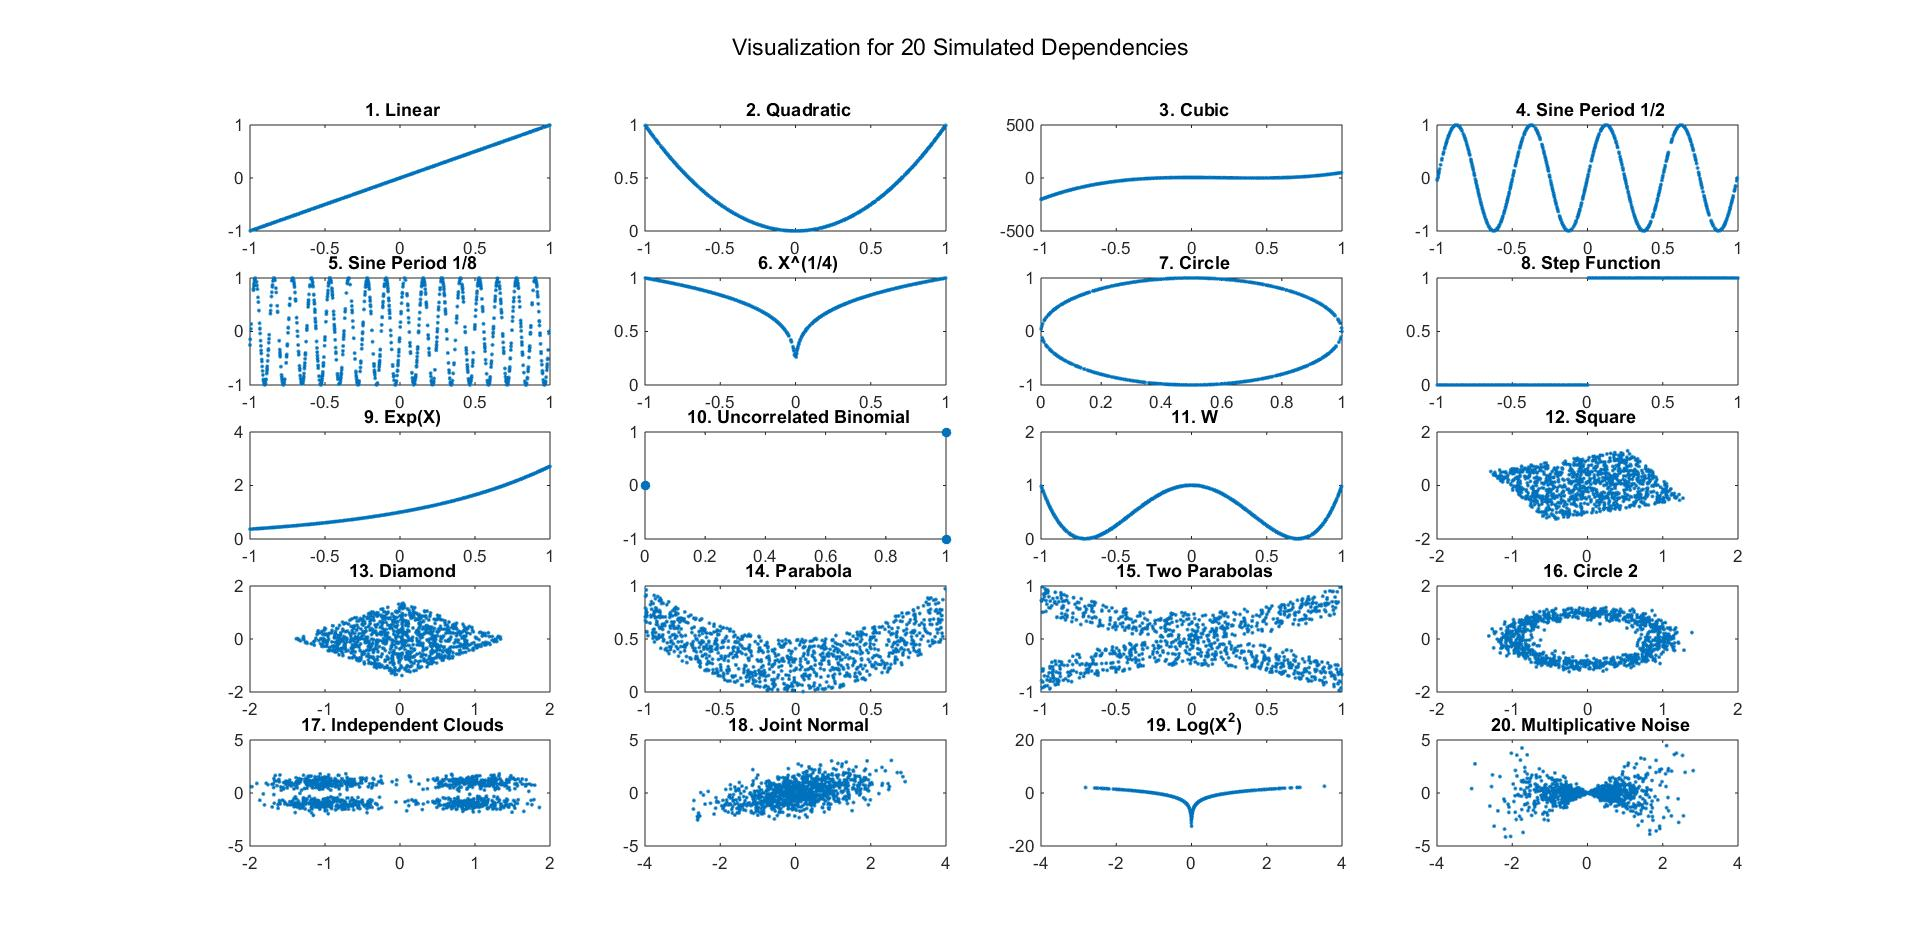
\includegraphics[width=1.0\textwidth]{Fig0.jpg}
	\caption{Visualization of $20$ Dependencies at $n=1000$ and Dimension $1$ with No Noise.}
	\label{fig1}
\end{figure} 
\end{frame}

\begin{frame}{Testing Powers at Dimension 1}
\begin{figure}[ht]
  \centering
  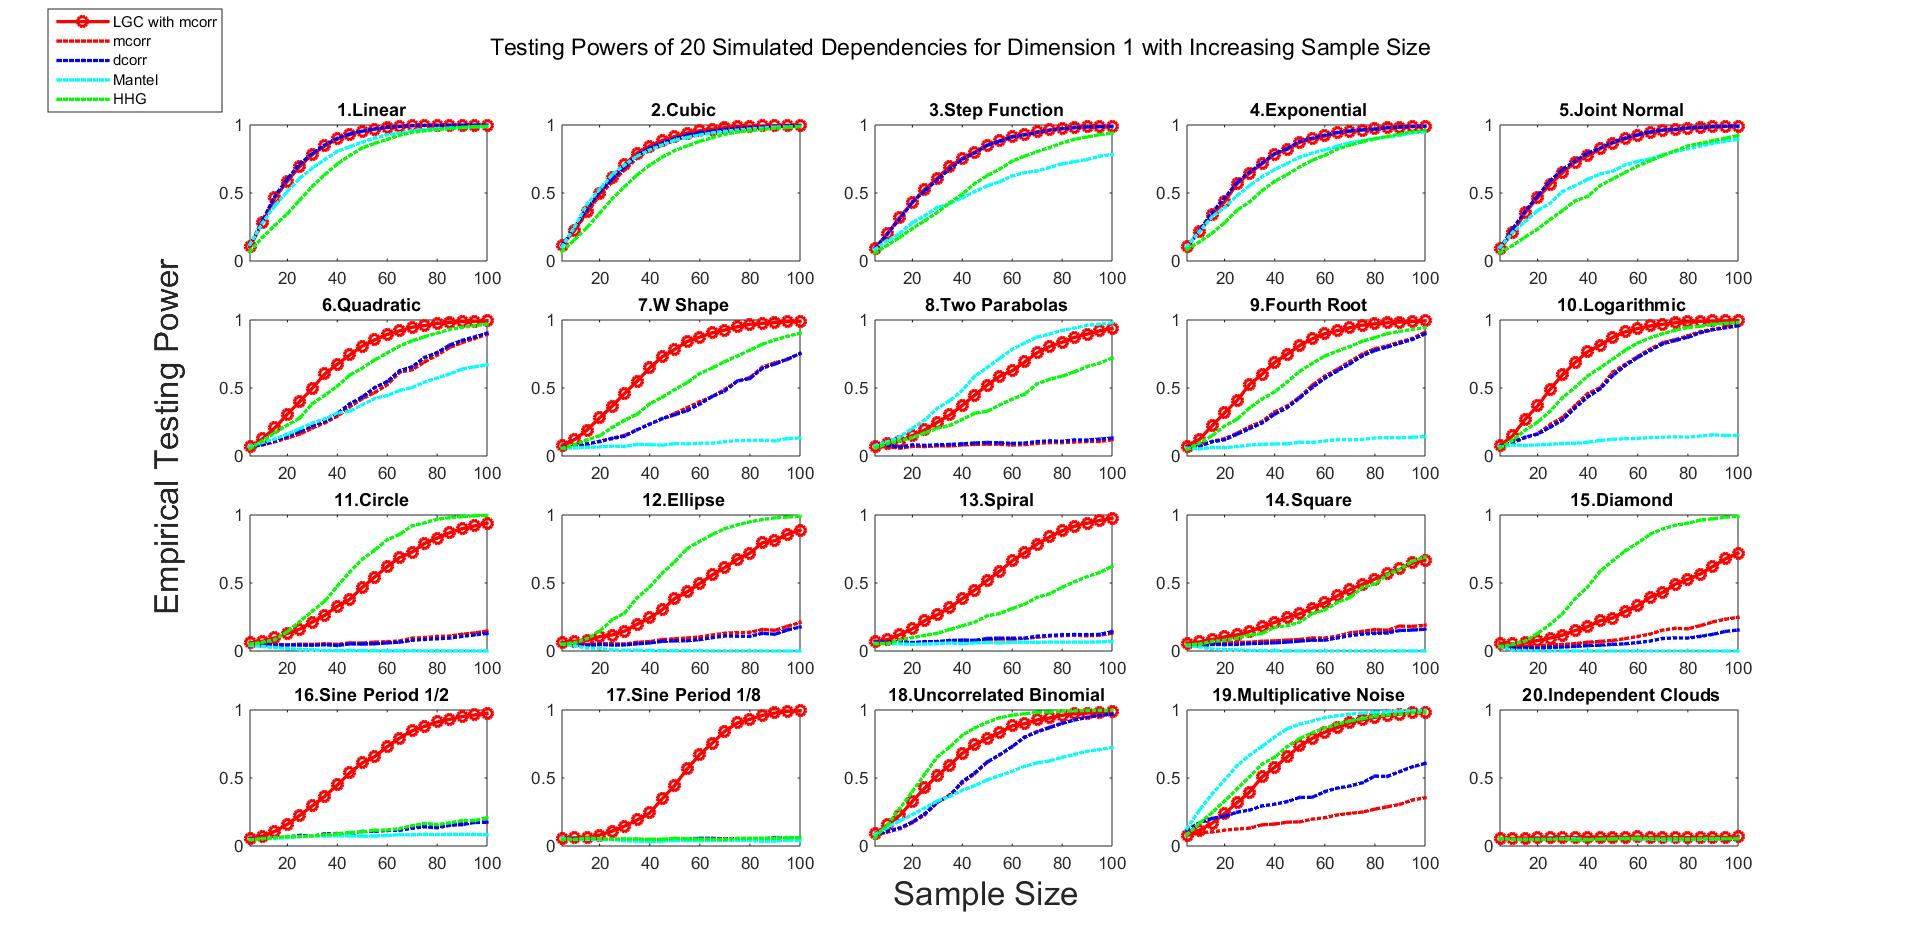
\includegraphics[width=1.0\textwidth]{Fig1.jpg}
	\caption{Testing Powers of Dimension 1 Simulations with Increasing Sample Size}
	\label{fig2}
\end{figure} 
\end{frame}

\begin{frame}{Performance Profiles at Dimension 1}
\begin{figure}[ht]
  \centering
  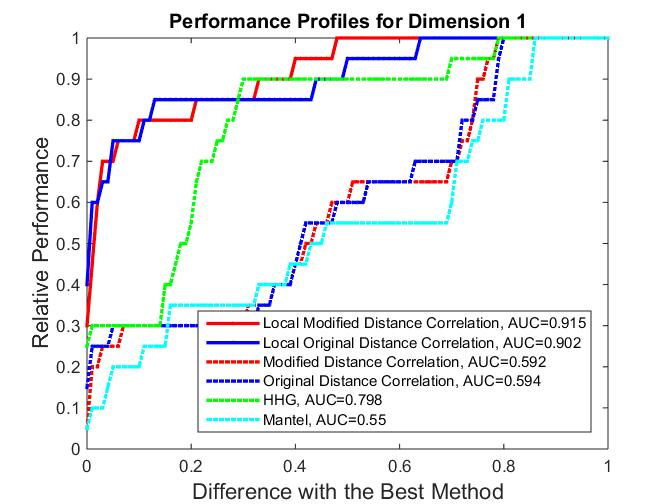
\includegraphics[width=0.8\textwidth]{Fig3.jpg}
	\caption{Performance Profiles of Dimension 1 Simulations}
	\label{fig3}
\end{figure} 
\end{frame}

\begin{frame}{Testing Powers of Increasing Dimension}
\begin{figure}[ht]
  \centering
  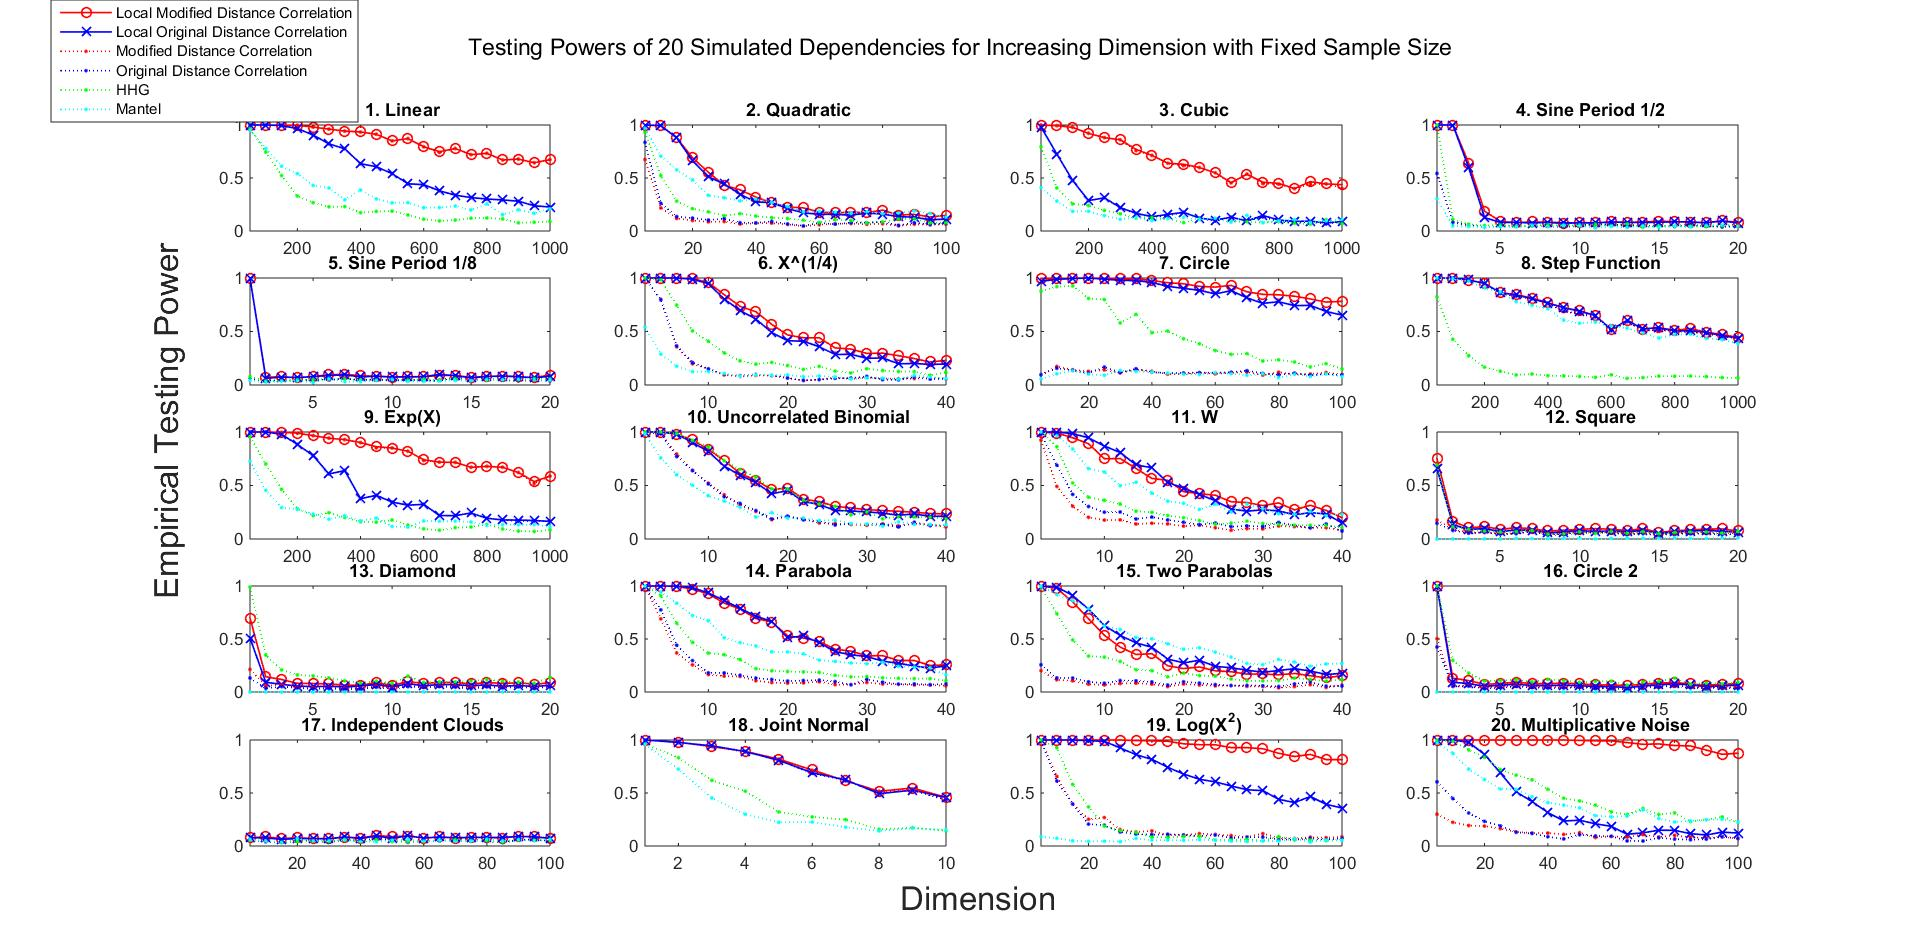
\includegraphics[width=1.0\textwidth]{Fig5.jpg}
	\caption{Testing Powers of Increasing Dimension Simulations with Fixed Sample Size}
\end{figure} 
\end{frame}

\begin{frame}{Performance Profiles of Increasing Dimension}
\begin{figure}[ht]
  \centering
  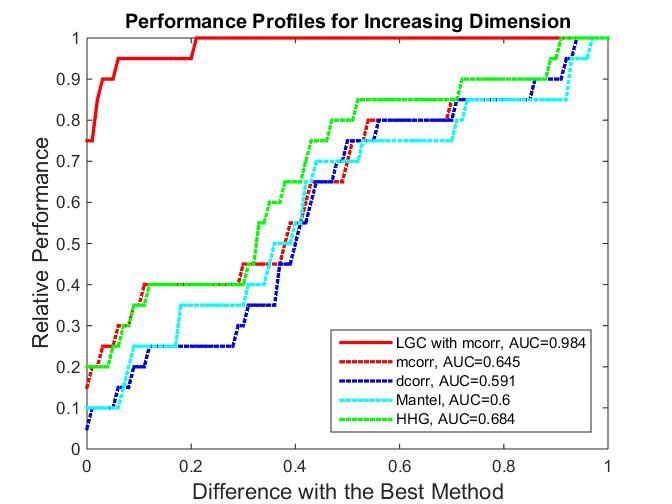
\includegraphics[width=0.8\textwidth]{Fig7.jpg}
	\caption{Performance Profiles of Increasing Dimension Simulations}
\end{figure} 
\end{frame}

\begin{frame}{P-Value of Real Data}
\begin{figure}[ht]
  \centering
  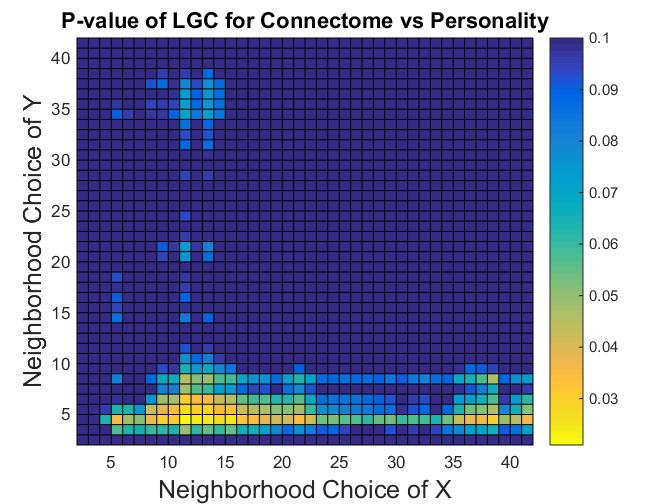
\includegraphics[width=0.8\textwidth]{FigReal1.jpg}
	\caption{P-Value of Brain Connectome and Personality}
\end{figure}
\end{frame}

\section{Conclusion}
\begin{frame}
\begin{itemize}[<+->]
\item We propose a local distance correlation to test independence.
\item It is not only theoretically consistent, but also achieves state-of-the-art performance in finite-sample testing of various dependencies.
\item Comparing to the benchmarks, it is overall the best method for testing data sets of linearity or non-linearity, high-dimensionality, and small sample-size.
\item It is able to detect signal in our real data! (Although the underlying truth is unknown)
\end{itemize}
\end{frame}

\begin{frame}{Potential Works}
\begin{itemize}[<+->]
\item The whole framework is applicable to Euclidean data/metric; but what about testing multiple graphs, or graph and other features?
\item Local distance correlation is potentially related to nonlinear embedding and its k-nearest-neighbor choice.
\item Other theoretical aspects/real-data applications of local distance correlation.
\item Move from testing independence to classification/prediction!
\end{itemize}
\end{frame}

%tba: add PIE and WIKI GF data
%\begin{frame}[allowframebreaks]
%\frametitle{References}
%\tiny
%\bibliographystyle{ieeetr}
%\bibliography{references}

%\end{frame}
\begin{frame}[allowframebreaks]

\frametitle{References}
\tiny
\bibliographystyle{ieeetr}
\bibliography{references}

\end{frame}

%------------------------------------------------

%----------------------------------------------------------------------------------------

\end{document} 
